\chapter{Plan de pruebas}
\label{sec:pruebas}

\section{Pruebas funcionales}

\subsection{Introducción}

El actual plan de pruebas tiene como objetivo asegurar que los requisitos especificados son cumplidos satisfactoriamente por el módulo de código implementado. Adicionalmente se buscará que el código implementado funcione correctamente cuando dispone de entradas incorrecta.

Este plan de pruebas, así como todos los creados como parte de este proyecto, está basado en el estándar IEEE 829 \cite{IEEE829}.

\subsection{Restricciones}

La principal restricción de este plan de pruebas es el tiempo. Sólo se dispone de 1 día para la creación del plan y otro día para su ejecución y la recolección de resultados.\\

La complejidad de las entradas que recibe el módulo limita el alcance de las pruebas de caja negra que podremos diseñar en el tiempo disponible.

\subsection{Objeto de pruebas}

El código a probar será la implementación del gestor de Spark, concretamente la clase {\it SolverManager\_PHSpark}. Su ejecución se realiza mediante el comando {\it runph} con la opción {\it -\-solver-manager=phspark}.\\

Se realizarán pruebas de caja negra sobre las diferentes opciones de configuración del solver manager. Adicionalmente se ejecutarán los ejemplos existentes en el proyecto y se comparará la solución generada mediante spark y mediante el algoritmo secuencial.

\subsection{Características a probar y exclusiones}

Se probarán las diferentes opciones de configuración que modifican la ejecución de phspark. Con esto verificamos el requisito RF-01 y RF-02.\\

Adicionalmente se ejecutan los ejemplos existentes para PySP mediante phspark y la implementación secuencial, comparando los resultados. De esta forma se verifica un funcionamiento correcto en distintos escenarios así como el requisito RF-03.\\

Queda excluído de este plan de pruebas la generación de pruebas mediante estrategias de caja blanca. No podremos asegurar una cobertura óptima de código pero no es posible realizarlas en el tiempo disponible dada la complejidad de las entradas.

\subsection{Estrategia}

Se utilizará el módulo ``unittest'' de Python para generar una clase que ejecute los casos de prueba diseñados.\\

Será necesario generar un archivo de salida correcto para usar como punto de comparación con las ejecuciones de pruebas. Será necesario filtrar las diferencais en la salida que causa la ejecución con Spark o, alternativamente, comprobar manualmente el resultado de cada pareja de archivos.

\subsection{Criterios de aceptación}

Se considerará que una prueba ha sido pasada correctamente si, tras introducir los datos de entrada escogidos, la aplicación devuelve una salida que concuerda exactamente con la que se estableció como esperada.\\

Será posible concluir que la aplicación aprobada pasó las pruebas si el 100\% de los casos válidos pasaron los criterios de aceptación. En caso contrario será necesaria la corrección de la implementación.

\subsection{Diseño de pruebas}

\TestItem[
    id={P-01},
    name={Conexión a Spark},
    requirements={RF-01, RF-02},
    objective={
        Valida la creación de una conexión a Spark.
    },
    techniques={
        \begin{itemize}
            \item \textbf{Por caja negra: }
            \begin{itemize}
                \item host
                \begin{itemize}
                    \item 1. Clase válida: Cadena que represente una IP correcta y disponible.
                    \item 2. Clase válida: Null.
                    \item 3. Clase no válida: Cadena que represente una IP errónea.
                    \item 4. Clase no válida: Cadena que represente una IP correcta pero no disponible.
                \end{itemize}
                \item port 
                \begin{itemize}
                    \item 5. Clase válida: Entero que represente un puerto correcto y disponible.
                    \item 6. Clase válida: Null.
                    \item 7. Clase no válida: Entero que represente un puerto erróneo.
                    \item 8. Clase no válida: Entero que represente un puerto correcto pero ocupado.
                \end{itemize}
            \end{itemize}
        \end{itemize}
    },
    testCases={CP-01, CP-02, CP-03, CP-04, CP-05, CP-06},
    expected={Conexión correcta y ejecución que genere la salida esperada en el caso de las pruebas para clases válidas. Para las pruebas con entradas no válidas se debe mostrar un error especificando el problema.}
]

\TestItem[
    id={P-02},
    name={Ejecución correcta de ejemplos},
    requirements={RF-01, RF-02, RF-03},
    objective={
        Valida que los resultados devueltos son correctos.
    },
    techniques={
        Se ejecutarán todos los ejemplos disponibles en \textit{``/pyomo/examples/pysp''} usando la versión secuencial para generar el resultado esperado y la versión Spark para verificar su funcionamiento.
    },
    testCases={CP-01, CP-02, CP-03},
    expected={Los resultados de todos los ejemplos son iguales para la versión secuencial y paralela.}
]

\subsection{Casos de prueba}

\TestCase[
    id={CP-01},
    description={Prueba la entrada correcta},
    validates={P-01(1,5)},
    environment={
        Instancia de Spark funcionando en ``spark://localhost:7077''
    },
    input={
        \makecell{
            host = ``localhost''\\
            port = 7077
        }
    },
    output={
        Igual a la ejecución con -\-solver-manager=serial
    }
]

\TestCase[
    id={CP-02},
    description={Prueba la url por defecto},
    validates={P-01(2,6)},
    environment={
        Instancia de Spark funcionando en ``spark://localhost:7077''
    },
    input={
        \makecell{
            host = None\\
            port = None
        }
    },
    output={
        Igual a la ejecución con -\-solver-manager=serial
    }
]

\TestCase[
    id={CP-03},
    description={Prueba la gestión de error al intentar conectarse a una IP incorrecta},
    validates={P-01(3)},
    environment={
        N/A
    },
    input={
        \makecell{
            host = ``111.111''\\
            port = None
        }
    },
    output={
        Mensaje de error indicando que no se ha podido conectar a Spark en la URL especificada.
    }
]

\TestCase[
    id={CP-04},
    description={Prueba la gestión de error al intentar conectarse a una IP donde no se está ejecutando Spark},
    validates={P-01(4)},
    environment={
        La URL ``spark://localhost:7077'' no debe tener ningún servicio escuchando.
    },
    input={
        \makecell{
            host = ``localhost''\\
            port = 7077
        }
    },
    output={
        Mensaje de error indicando que no se ha podido conectar a Spark en la URL especificada.
    }
]

\TestCase[
    id={CP-05},
    description={Prueba la gestión de error al especificar un puerto inválido},
    validates={P-01(7)},
    environment={
        N/A
    },
    input={
        \makecell{
            host = None\\
            port = -1
        }
    },
    output={
        Mensaje de error indicando que no se ha podido conectar a Spark en la URL especificada.
    }
]

\TestCase[
    id={CP-06},
    description={Prueba la gestión de error al especificar un puerto donde no se está ejecutando Spark},
    validates={P-01(8)},
    environment={
        La URL ``spark://localhost:8080'' no debe ser una instancia de Spark
    },
    input={
        \makecell{
            host = ``localhost''\\
            port = 8080
        }
    },
    output={
        Mensaje de error indicando que no se ha podido conectar a Spark en la URL especificada.
    }
]

\subsection{Procedimiento de pruebas}

Los casos de prueba especificados son idempotentes y no es necesario especificar un orden concreto para su ejecución. Será necesario para cada uno establecer el entorno especificado en cada caso concreto. Adicionalmente, para verificar los resultados será necesario ejecutar la misma entrada de forma secuencial para comparar.\\

Para la prueba P-02 no se especifican casos de prueba concretos porque todos se ejecutan de la misma forma cambiando el directorio de entrada. Para esta prueba se ejecutarán todos los ejemplos disponibles para PySP de forma secuencial y, posteriormente, usando Spark. Si Spark devuelve siempre los mismos resultados (dentro de un margen de error) se considerará la prueba como superada.

\subsection{Ejecución de las pruebas}

Por limitaciones temporales, los tests unitarios no están totalmente automatizados. Actualmente, la arquitectura de tests necesita de la creación de archivos de referencia para contrastar con la salida de la ejecución de prueba. Adicionalmente, por las posibles diferencias entre ambos archivos no relevantes para el resultado (como mensajes informativos), se debe programar un filtro concreto para las diferentes salidas.\\

Por las razones expuestas los tests se programarán para ejecutarse automáticamente, pero se debe comprobar manualmente si la salida es la esperada. Para realizar esta comprobación se ejecutará el mismo comando que ejecuta cada test, pero utilizando {\it --solver-manager=serial}.\\

La solución de cada ejecución se guarda en un archivo \textit{ph\_solution.json}. Se guarda la solución de la ejecución secuencial y posteriormente es posible ejecutar \textit{diff} con la solución devuelta por el test, siempre que se espere una salida correcta. En caso contrario se comprobará manualmente que la salida es la esperada.\\

\begin{tabularx}{\linewidth}{|c|X|c|}
    \hline
    \textbf{ID} & \centering \textbf{Salida} & \textbf{Superada} \tabularnewline
    \hline
    CP-01 & TestPHFarmerSpark.test1.ph\_solution.json.out & Si \tabularnewline
    \hline
    CP-02 & TestPHFarmerSpark.test2.ph\_solution.json.out & Si \tabularnewline
    \hline
    CP-03 & RuntimeError: ERROR connecting with Spark at spark://111.111:7077. URL might be incorrect (org.apache.spark.SparkException)Invalid master URL: spark://111.111:7077 & Si \tabularnewline
    \hline
    CP-04 & RuntimeError: ERROR connecting with Spark at spark://192.10.10.10:7077. Check if Spark is running on that IP. (java.lang.IllegalArgumentException)requirement failed: Can only call getServletHandlers on a running MetricsSystem & Si \tabularnewline
    \hline
    CP-05 & RuntimeError: ERROR connecting with Spark at spark://localhost:-1. URL might be incorrect (org.apache.spark.SparkException)Invalid master URL: spark://localhost:-1 & Si \tabularnewline
    \hline
    CP-06 & RuntimeError: ERROR connecting with Spark at spark://localhost:8080. Check if Spark is running on that IP. (java.lang.IllegalArgumentException)requirement failed: Can only call getServletHandlers on a running MetricsSystem & Si \tabularnewline
    \hline
\end{tabularx}

A continuación se probará la ejecución de los ejemplos disponibles en el proyecto. Para ello se utilizará un script en bash que se mueva entre los directorios y ejecute la versión secuencial y paralela para cada ejemplo, imprimiendo los resultados de ejecutar el comando \textit{diff}. Aunque con este script se busca automatizar al máximo la ejecución de pruebas, no se consigue totalmente. La naturaleza del algoritmo hace que existan ligeras diferencias en los valores generados. Esto causará que las salidas sean diferentes, pero no implica que los resultados sean incorrectos. 
Para facilitar la comprobación de esta situación, se utiliza la herramienta \textit{colordiff} que resaltará las diferencias entre ambas soluciones.\\

A continuación se muestra el primer test del script donde se ejecuta el ejemplo ``Farmer''. La ejecución de los ejemplos restantes es equivalente, modificando únicamente las rutas de los archivos.\\

\begin{figure}[H]
    \centerline{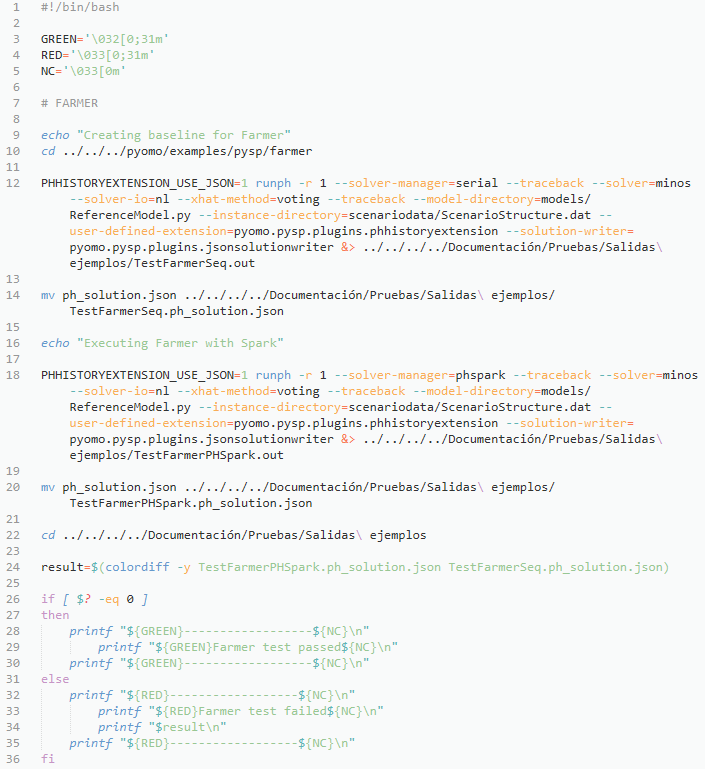
\includegraphics[width=15cm]{figuras/codigo/script-pruebas.png}}
    \caption{Script de pruebas}
\end{figure}

El resultado de ejecutar este script completo se muestra en la tabla a continuación: \\

\begin{tabularx}{\linewidth}{|X|c|}
    \hline
    Farmer & passed \tabularnewline
    \hline
    Baa99 & failed (stackoverflow) \tabularnewline
    \hline
    Farmer\_generated & failed (stackoverflow) \tabularnewline
    \hline
    FarmerWIntegers & passed \tabularnewline
    \hline
    FarmerWPieceWise & passed \tabularnewline
    \hline
    FarmerWrent & passed \tabularnewline
    \hline
    Finance & failed (stackoverflow) \tabularnewline
    \hline
    Hydro & passed \tabularnewline
    \hline
\end{tabularx}
\\ \newline
Podemos observar que algunos tests aparecen como fallidos con un error \textit{stackoverflow}. Esto no significa necesariamente que el programa no funcione como se espera, lo más probable es que se deba a limitaciones de la máquina en la que se han realizado las pruebas.\\

Queda como tarea en un futuro optimizar la gestión de la memoria y el uso de Spark para que ejecutar problemas como este sea posible en máquinas con menos recursos. 

\section{Pruebas de rendimiento}

\subsection{Introducción}

Este segundo plan de pruebas se centrará en evaluar el rendimiento de la implementación con Spark. El objetivo es establecer una medición concreta comparando la ejecución en Spark con la ejecución secuencial y con Pyro.

\subsection{Restricciones}

Existen dos restricciones principales sobre la realización de este plan de pruebas. En primer lugar, el tiempo disponible. Se disponen de 3 días para elaborar, ejecutar y analizar las pruebas expuestas en esta sección. \\

Adicionalmente, las pruebas no se ejecutarán en un cluster de computación, lo que limitará el tamaño de los problemas a probar y la escalabilidad que podremos observar. La máquina de pruebas será un portátil ejecutando una máquina virtual con las siguientes características:

\begin{itemize}
    \item Fedora 27 (Workstation Edition)
    \item i7 7700HQ
    \item 4GB
\end{itemize}

\subsection{Objeto de pruebas}

Durante la ejecución del primer plan de pruebas se realizaron mediciones en el tiempo de ejecución de los ejemplos existentes como parte de Pyomo. Con estos valores iniciales decidimos que se utilizará el ejemplo ``Hydro'' para esta evaluación de rendimiento. Este ejemplo nos proporciona un problema con 9 escenarios, lo que debería favorecer la escalabilidad en paralelo, y se puede ejecutar en un tiempo razonable en nuestra máquina de pruebas.

\subsection{Características a probar y exclusiones}

Se medirá el tiempo de ejecución del ejemplo especificado utilizando diferentes configuraciones hardware, usando desde 1 núcleo hasta 8 para Spark y con variaciones en la memoria disponible.

\subsection{Estrategia}

Se utilizará la opción `\textit{--output-times}' que utiliza la librería ``time'' de python para la medición de tiempos. Los valores de las diferentes ejecuciones se recopilarán en una hoja de cálculo para generar gráficas que faciliten el estudio de los resultados.

\subsection{Criterios de aceptación}

Las pruebas se considerarán satisfactorias si producen resultados estudiables. Dichos resultados deben ser replicables utilizando una configuración similar. Deben evitarse resultados que pueden haber sido alterados por condiciones externas durante la ejecución del programa, por lo que deberían realizarse múltiples ejecuciones iguales para filtrar los resultados coherentes.

\subsection{Casos de prueba}

En este plan de pruebas no definiremos casos de prueba siguiendo el estándar. A continuación se listan las diferentes configuraciones de núcleos y memoria con las que realizará la ejecución.

\begin{tabularx}{\linewidth}{|X|X|}
    \hline
    \centering \textbf{Hilos} & \centering \textbf{Memoria} \tabularnewline
    \hline
    \centering 1 & \centering 2GB \tabularnewline
    \hline
    \centering 2 & \centering 2GB \tabularnewline
    \hline
    \centering 3 & \centering 2GB \tabularnewline
    \hline
    \centering 4 & \centering 2GB \tabularnewline
    \hline
    \centering 5 & \centering 2GB \tabularnewline
    \hline
    \centering 6 & \centering 2GB \tabularnewline
    \hline
    \centering 7 & \centering 2GB \tabularnewline
    \hline
    \centering 8 & \centering 2GB \tabularnewline
    \hline
    \centering 1 & \centering 4GB \tabularnewline
    \hline
    \centering 2 & \centering 4GB \tabularnewline
    \hline
    \centering 3 & \centering 4GB \tabularnewline
    \hline
    \centering 4 & \centering 4GB \tabularnewline
    \hline
    \centering 5 & \centering 4GB \tabularnewline
    \hline
    \centering 6 & \centering 4GB \tabularnewline
    \hline
    \centering 7 & \centering 4GB \tabularnewline
    \hline
    \centering 8 & \centering 4GB \tabularnewline
    \hline       
\end{tabularx}

\subsection{Procedimiento de pruebas}

Utilizando las configuraciones anteriores se ejecutará cada una de ellas 3 veces y se guardará una media de los tiempos.\\

Se establecerá también la media de duración por iteración para observar de forma más concreta el overhead causado por la nueva implementación.

\subsection{Ejecución de las pruebas}

El primer aspecto a probar es el tiempo de ejecución del ejemplo \textit{Hydro}. Este modelo especifica 9 escenarios diferentes que, teniendo en cuenta que la paralelización se realiza a nivel de escenario, es esperable una buena escalabilidad.\\

Sin embargo, los resultados obtenidos no cumplen lo esperado:\\

\begin{figure}[H]
    \centerline{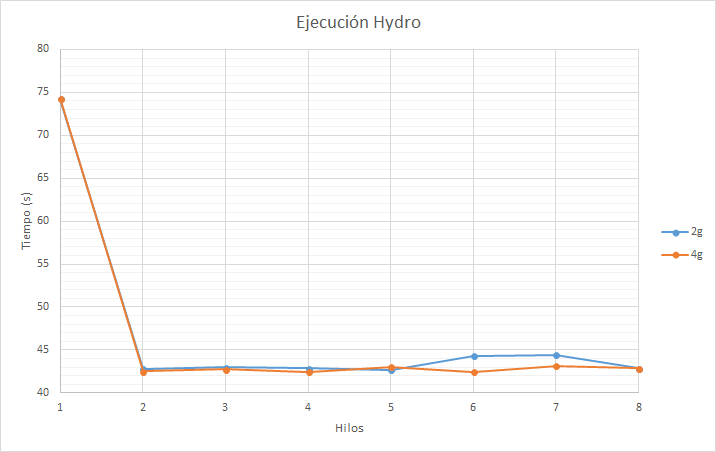
\includegraphics[width=15cm]{figuras/pruebas/test-hydro.png}}
    \caption{Tiempos de ejecución Hydro}
    \label{fig:test-hydro}
\end{figure}

Para analizar estos datos, primero debemos tener en cuenta dos puntos importantes: la ejecución no se ha realizado en una máquina adecuada para aprovechar la paralelización y el tiempo de ejecución de la versión secuencia es de aproximadamente 6s.\\

A parte de ejecutar las pruebas con distinto número de hilos, también se ha probado a limitar la memoria disponible en Spark a 2GB o 4GB. Esto está representado en la gráfica como las líneas naranja y azul. Podemos concluir facilmente que, para este ejemplo concreto, no existe diferencia en la memoria disponible. Esto puede ser porque la memoria necesaria es siempre inferior a 2GB o es siempre superior a 4GB. \\

En cuanto a los tiempos de ejecución, si tenemos en cuenta que la ejecución normal tarda unos 6s, la implementación con Spark utilizando 1 hilo tarda 74s, siendo una opción claramente peor a nivel temporal.\\

Aumentando el número de hilos disponible, observamos inicialmente una mejora importante. Pasando de 1 a 2 hilos reducimos el tiempo casi a la mitad (0,57x). Esto es una prueba de la escalabilidad que promete Spark. Sin embargo, aumentar el número de hilos no resulta en ningún tipo de mejora, a pesar de que esperábamos mejoras con la utilización de hasta 9 hilos (por existir 9 escenarios). Esto puede ser el resultado de ejecutar un programa demasiado pequeño en una plataforma poco adecuada. \\

Estos tiempos están claramente lejos de lo conseguido con la ejecución secuencial, pero son un claro indicador del potencial de una implementación con Spark para la resolución de problemas estocásticos y, con futuras optimizaciones y un cluster donde ejecutarse, esta implementación podría ser una alternativa viable para abordar problemas que antes no eran resolubles en un tiempo razonable.\\

Con el objetivo de analizar los tiempos sobre un problema mayor se utilizarán los tiempos establecidos por el ejemplo \textit{Finance}. Este ejemplo no consigue finalizar por lo que parecen ser limitaciones de memoria, pero sí podemos observar los tiempos de ejecución de las primeras iteraciones. Se seleccionan los tiempos de ejecución de las primeras 10 iteraciones y se hace una media de los mismos. En la siguiente figura se muestra el tiempo medio por iteración para el ejemplo \textit{Finance} así como para el anterior ejemplo \textit{Hydro} utilizando 1,2 y 8 hilos.\\

\begin{figure}[H]
    \centerline{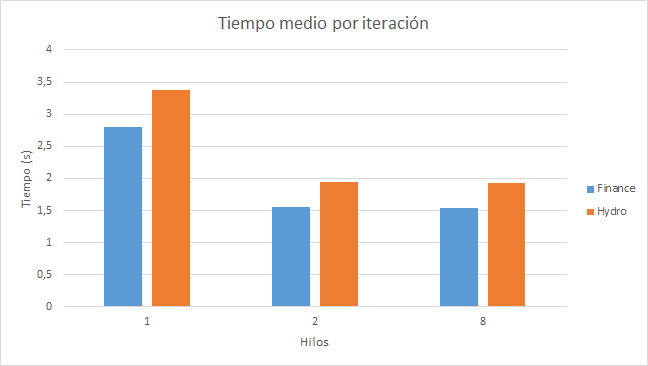
\includegraphics[width=15cm]{figuras/pruebas/test-iteration-time.png}}
    \caption{Tiempo medio por iteración}
    \label{fig:test-iteration-time}
\end{figure}

Los resultados, de nuevo, no son los esperados. El ejemplo \textit{Finance} no falla porque el modelo a procesar sea demasiado grande, si no porque necesita una mayor cantidad de datos durante más iteraciones. \\

En esta prueba observamos un comportamiento similar a lo visto en la anterior gráfica. En primer lugar, el ejemplo \textit{Finance} se ejecuta más rápido que \textit{Hydro} y conseguimos una mejora del 0,55x y 0,57x respectivamente. 